\documentclass[justified]{tufte-handout}
\usepackage{../braph2_tut}
%\geometry{showframe} % display margins for debugging page layout

\title{Pipeline for Comparison of Connectivity Data using Binary Undirected graphs at fixed Thresholds}

\begin{document}

\maketitle

\begin{abstract}
\noindent
In this tutorial, we will upload a file containing the pipeline with the different steps to compare two groups of subjects using \emph{connectivity data} (check tutorial \emph{Group of Subjects with Connectivity Data}) and binary undirected graphs at fixed thresholds. This Tutorial explains how to perform group analyses and comparisons with this kind of data.
\end{abstract}

\tableofcontents

\fig{figure*}
	{fig:01}
	{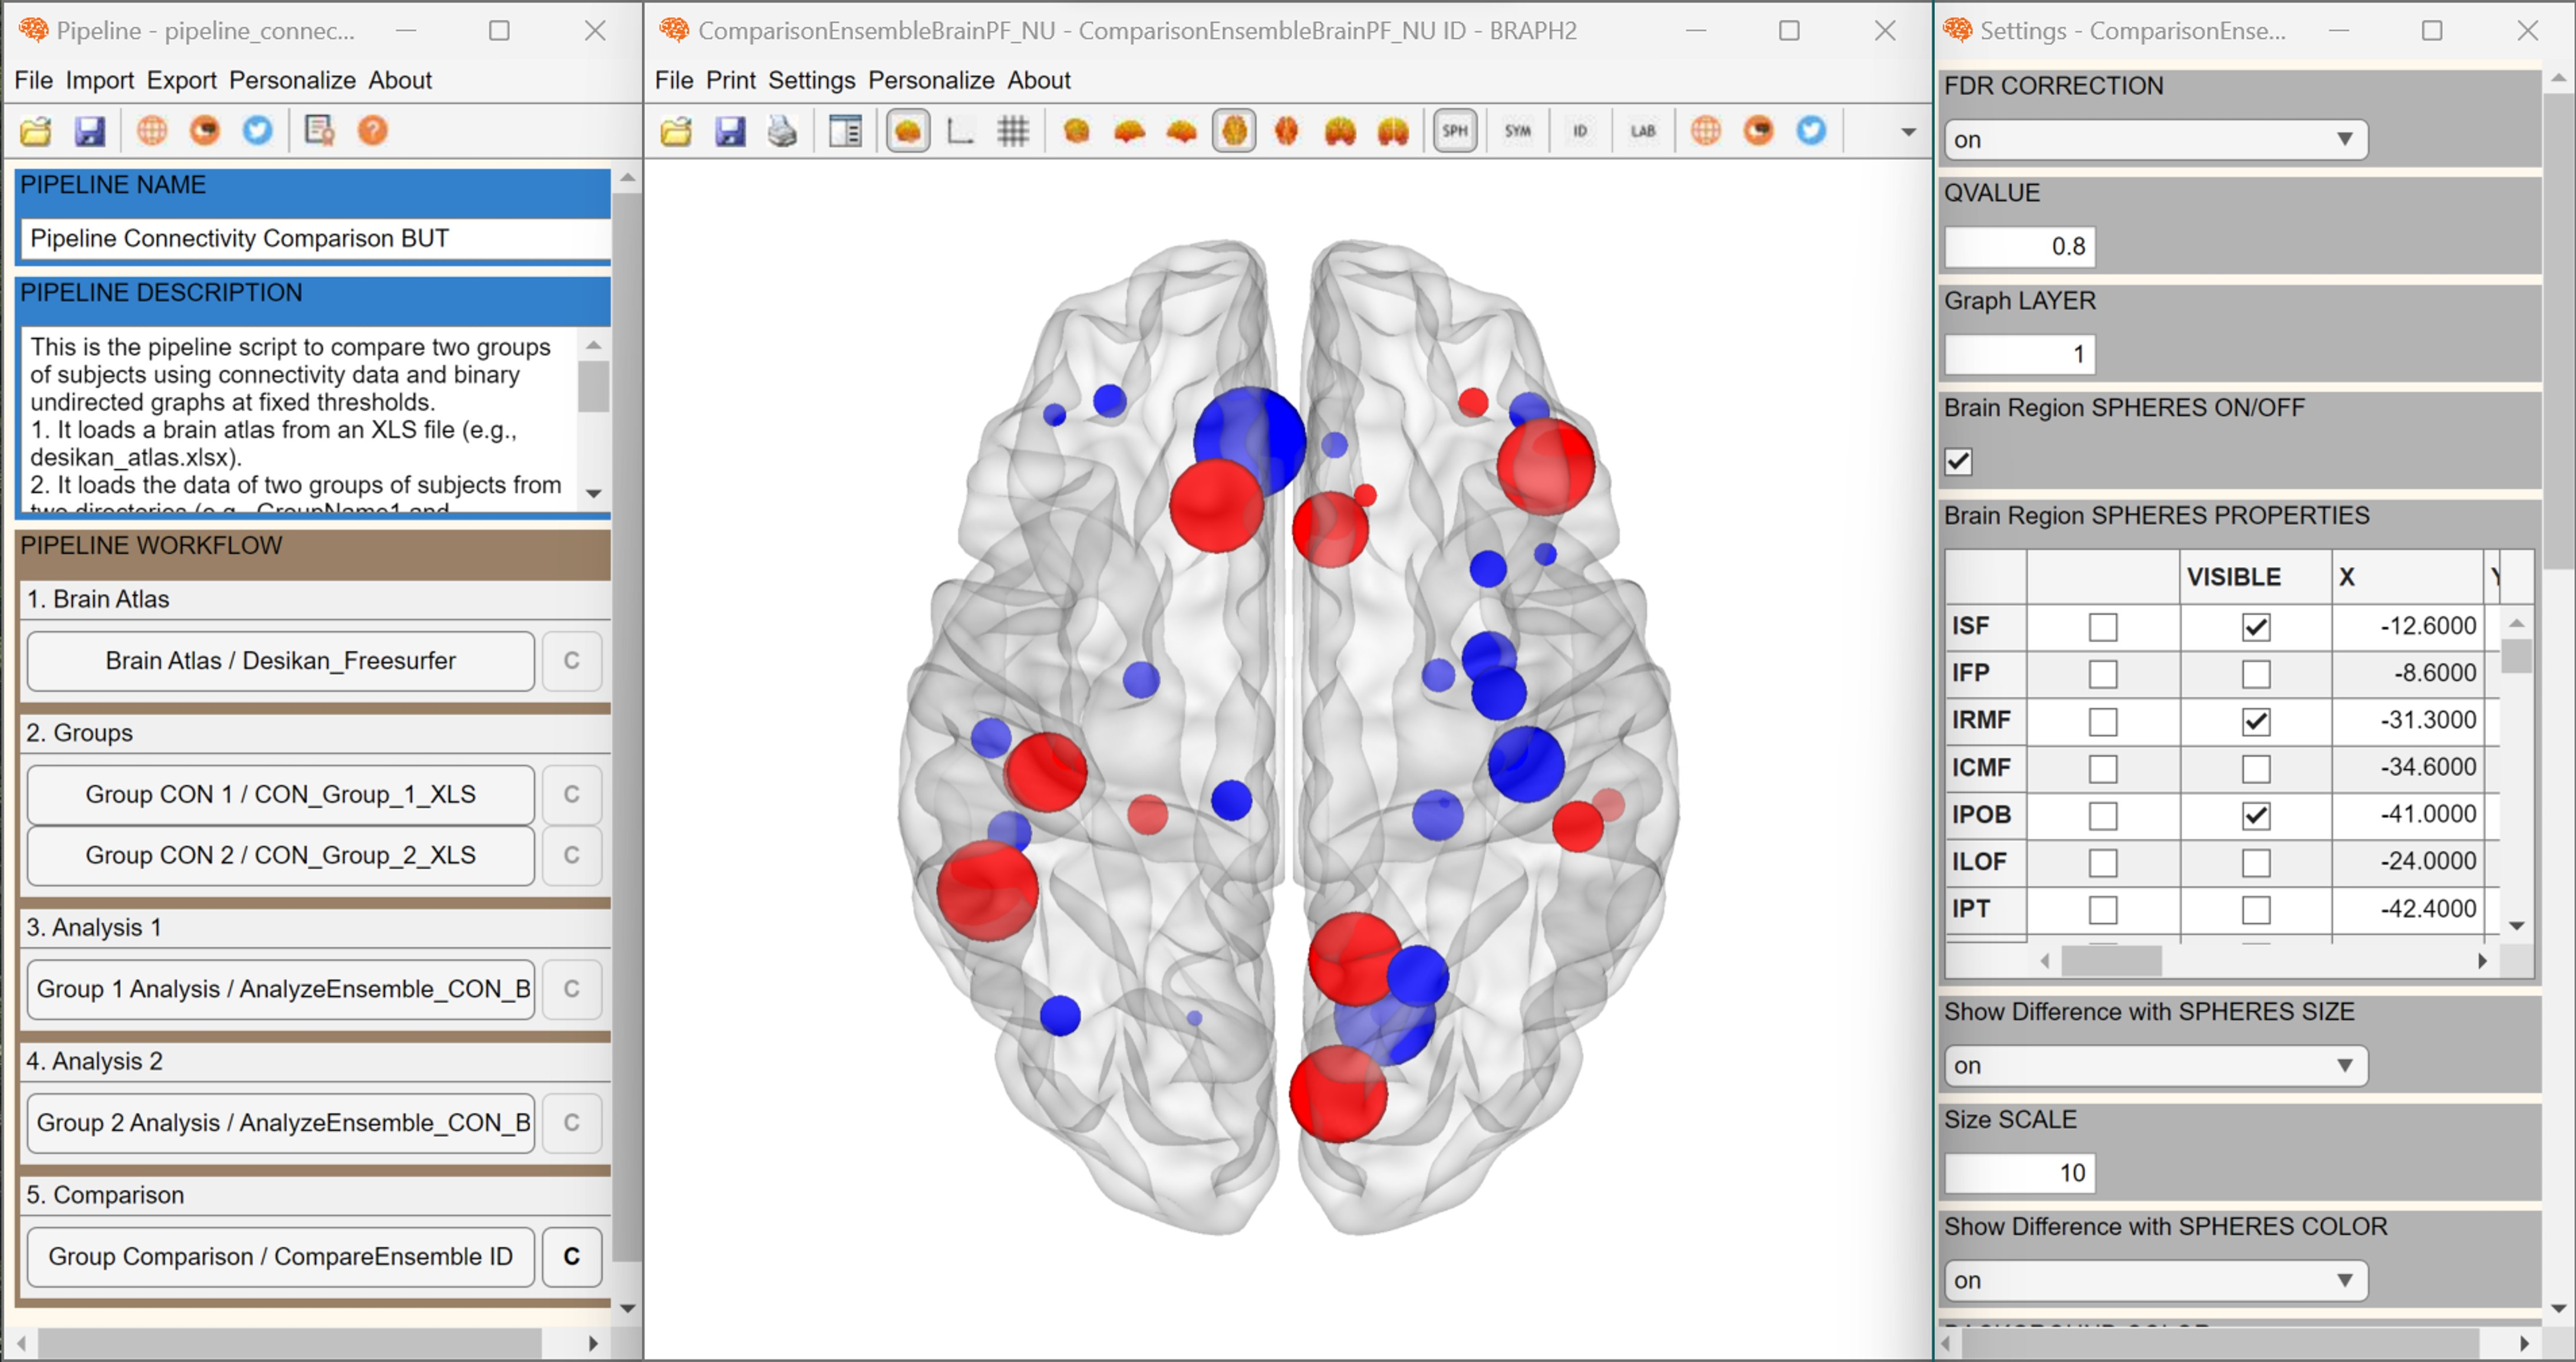
\includegraphics{fig01.jpg}}
	{GUI for working with the pipeline to compare two groups of subjects with \emph{connectivity data} using binary undirected graphs at fixed thresholds.}
	{
	Full graphical user interface to perform group comparisons with \emph{connectivity data} in BRAPH~2.0. 
	}

\clearpage
\section{Open the GUI}

The pipeline GUI can be opened by typing \code{braph2} in MatLab's terminal, which allows you to select a pipeline, in this case, \fn{pipeline\_connectivity\_comparison\_but.braph2} (containing the steps required to perform your analysis).

To open the GUI and upload the connectivity comparison pipeline, you can also do it from the command line by typing the commands in \Coderef{cd:launch}.
%
\begin{lstlisting}[
	label=cd:launch,
	caption={
		{\bf Code to launch the GUI to upload a pipeline file to compare two groups of subjects.}
		This code can be used in the MatLab command line to launch the GUI to upload a pipeline file.
	}
]
pip = Pipeline(); ¥\circled{1}\circlednote{1}{creates a new object \code{Pipeline} to upload the steps to perform an analysis or comparison.}¥

gui = GUIElement('PE', pip); ¥\circled{2}\circlednote{2}{creates a GUI to upload the files into the pipeline.}¥
gui.get('DRAW')¥\circled{3}\circlednote{3}{draws the GUI.}¥
gui.get('SHOW') ¥\circled{4}\circlednote{4}{shows the GUI.}¥
\end{lstlisting}

Once the pipeline is uploaded, you can see a GUI that contains different steps: to upload a brain atlas, to upload the structural data of two groups, analyze them, and finally, to compare the groups (\Figref{fig:03}a). 

\section{Step 1: Load the Brain Atlas}

\Figref{fig:03} shows how to upload the brain atlas that you used to extract the connectivity data for your analysis.

\fig{figure}
	{fig:03}
	{
	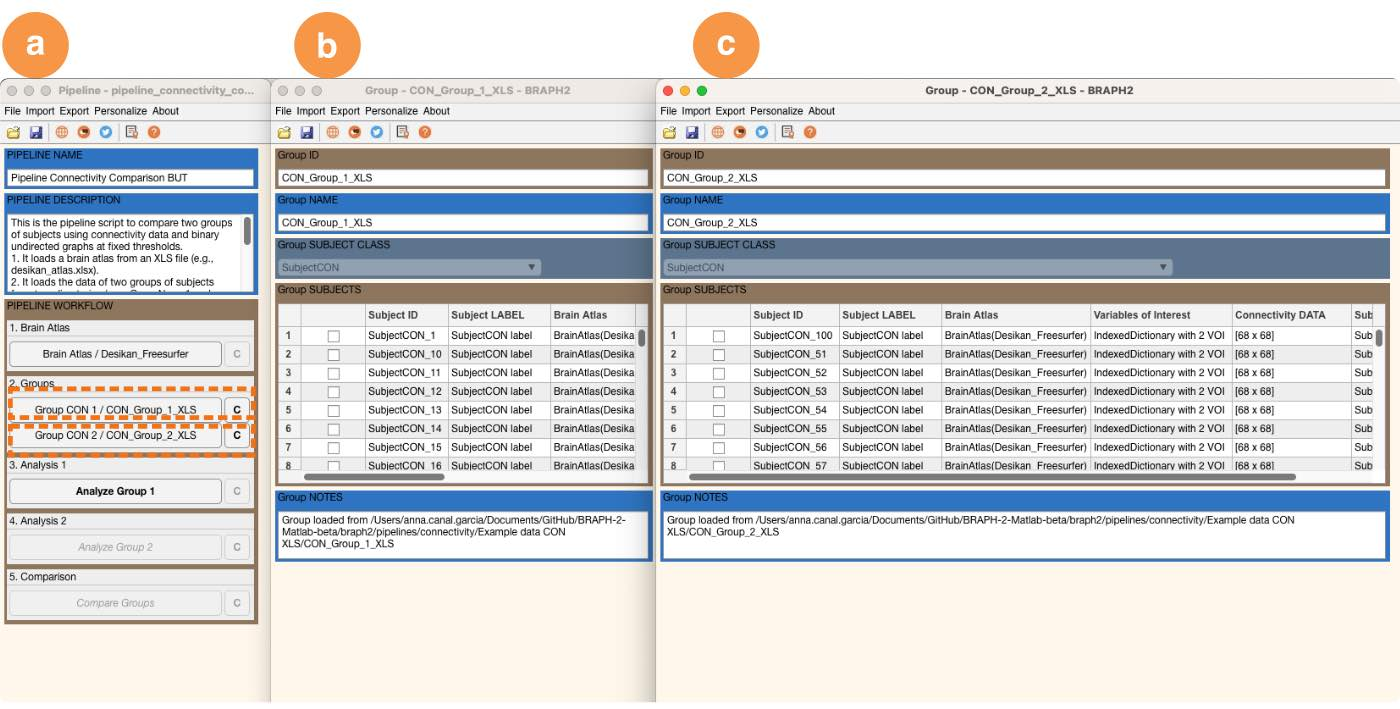
\includegraphics{fig03.jpg}
	}
	{Uploading the Brain Atlas}
	{
	Steps to upload the brain atlas:
	{\bf a} Click on \fn{Load Atlas} from the pipeline GUI.
	{\bf b} Navigate to the BRAPH~2.0 folder \fn{atlases} and {\bf c} select one of the atlas files, in this example the \fn{destrieux\_atlas.xlsx}. Similarly to the other tutorials, you can edit the information of this atlas as desired, including the Brain Atlas ID, NAME, NOTES or Brain Regions. You can also plot the brain atlas and visualize it using different options.
	}
 
\section{Step 2: Load the Structural Group Data}

After you loaded the brain atlas, you can upload the structural data for each group as shown in \Figref{fig:04}. A new interface will be shown containing the data for the group you just selected. You can open each subject’s structural values by selecting
the subject, right click, and select “Open selection” (\Figref{fig:04}f), which shows these values (\Figref{fig:04}g). 
	
	\fig{figure}
	{fig:04}
	{
	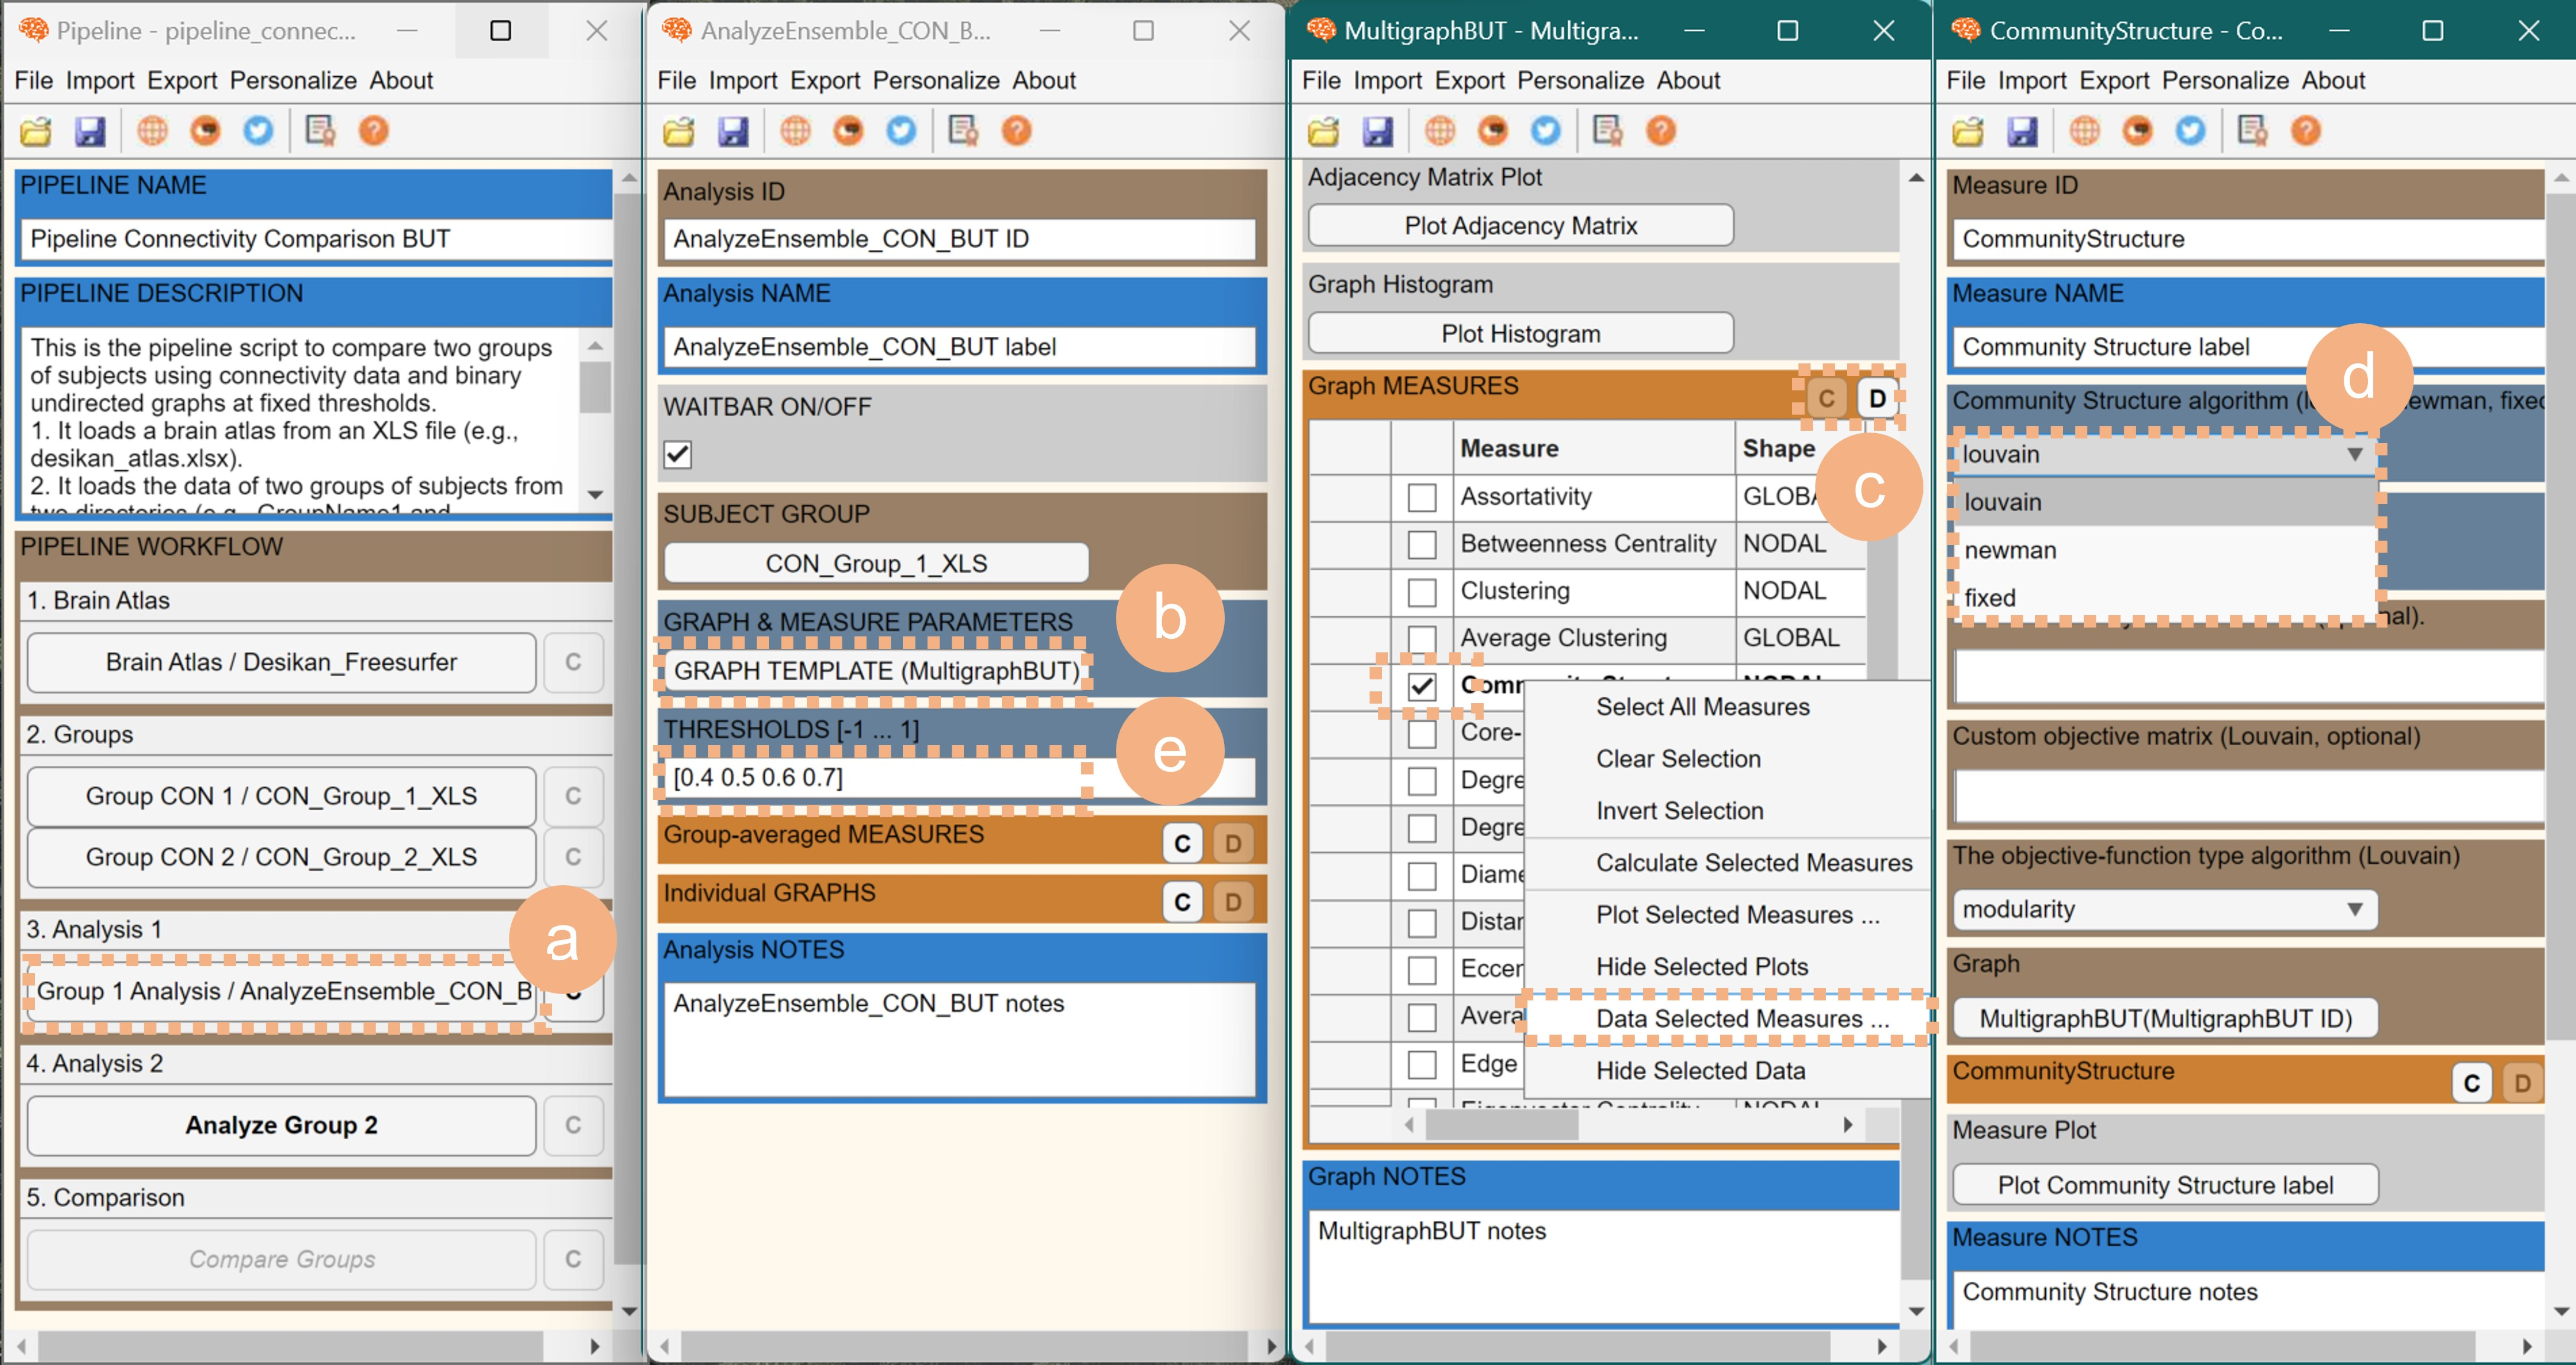
\includegraphics{fig04.jpg}
	}
	{Loading the Group Data}
	{
	Steps to upload the data from each group:
	{\bf a} Click on \fn{Load Group ST XLS from the pipeline GUI}.
	{\bf b} Navigate to the BRAPH~2.0 folder \fn{pipelines}, {\bf c} \fn{structural}, {\bf d} \fn{Example data ST XLS}, and select the file {\bf e} \fn{ST\_Group\_1\_.xlsx}.
	}
You should repeat the same procedure for group 2.

\section{Step 3: Analysing the Data of Group 1}

After you have loaded the data, you can analyze the data of your first group by clicking on \fn{Analyze Group 1} (\Figref{fig:05}a). A new interface will be shown that allows you to pre-calculate network measures for each group and explore them (\Figref{fig:05}b). First of all, you can specify the parameters for constructing the graph from the structural group data: you can select the statistical test to calculate correlations in structural values between pairs of brain regions (\Figref{fig:05}c), and you can decide how you want to analyze the negative weights from the correlation (\Figref{fig:05}d). After setting these parameters, you can calculate some graph measures (\Figref{fig:05}e), which might be useful to get an insight on what these measures look like for the group. Once calculated, the graph parameters will be blocked and a C will appear next to the measures. You can visualize the results by selecting the measures, right click and plot the selected measures. In settings you can change the visualization of the plots and save them. When you do right click there are other options you can explore such as Plot Graph Plot (connectivity matrix) as well as Data Graph (labels of brain regions, values of the adjacency matrix, options to plot matrix and histogram), all of which can also be saved.

Importantly, the parameters you select for this analysis (graph and measures parameters) will be fixed for the analysis of the second group and for the group comparisons.

	\fig{figure}
	{fig:05}
	{
	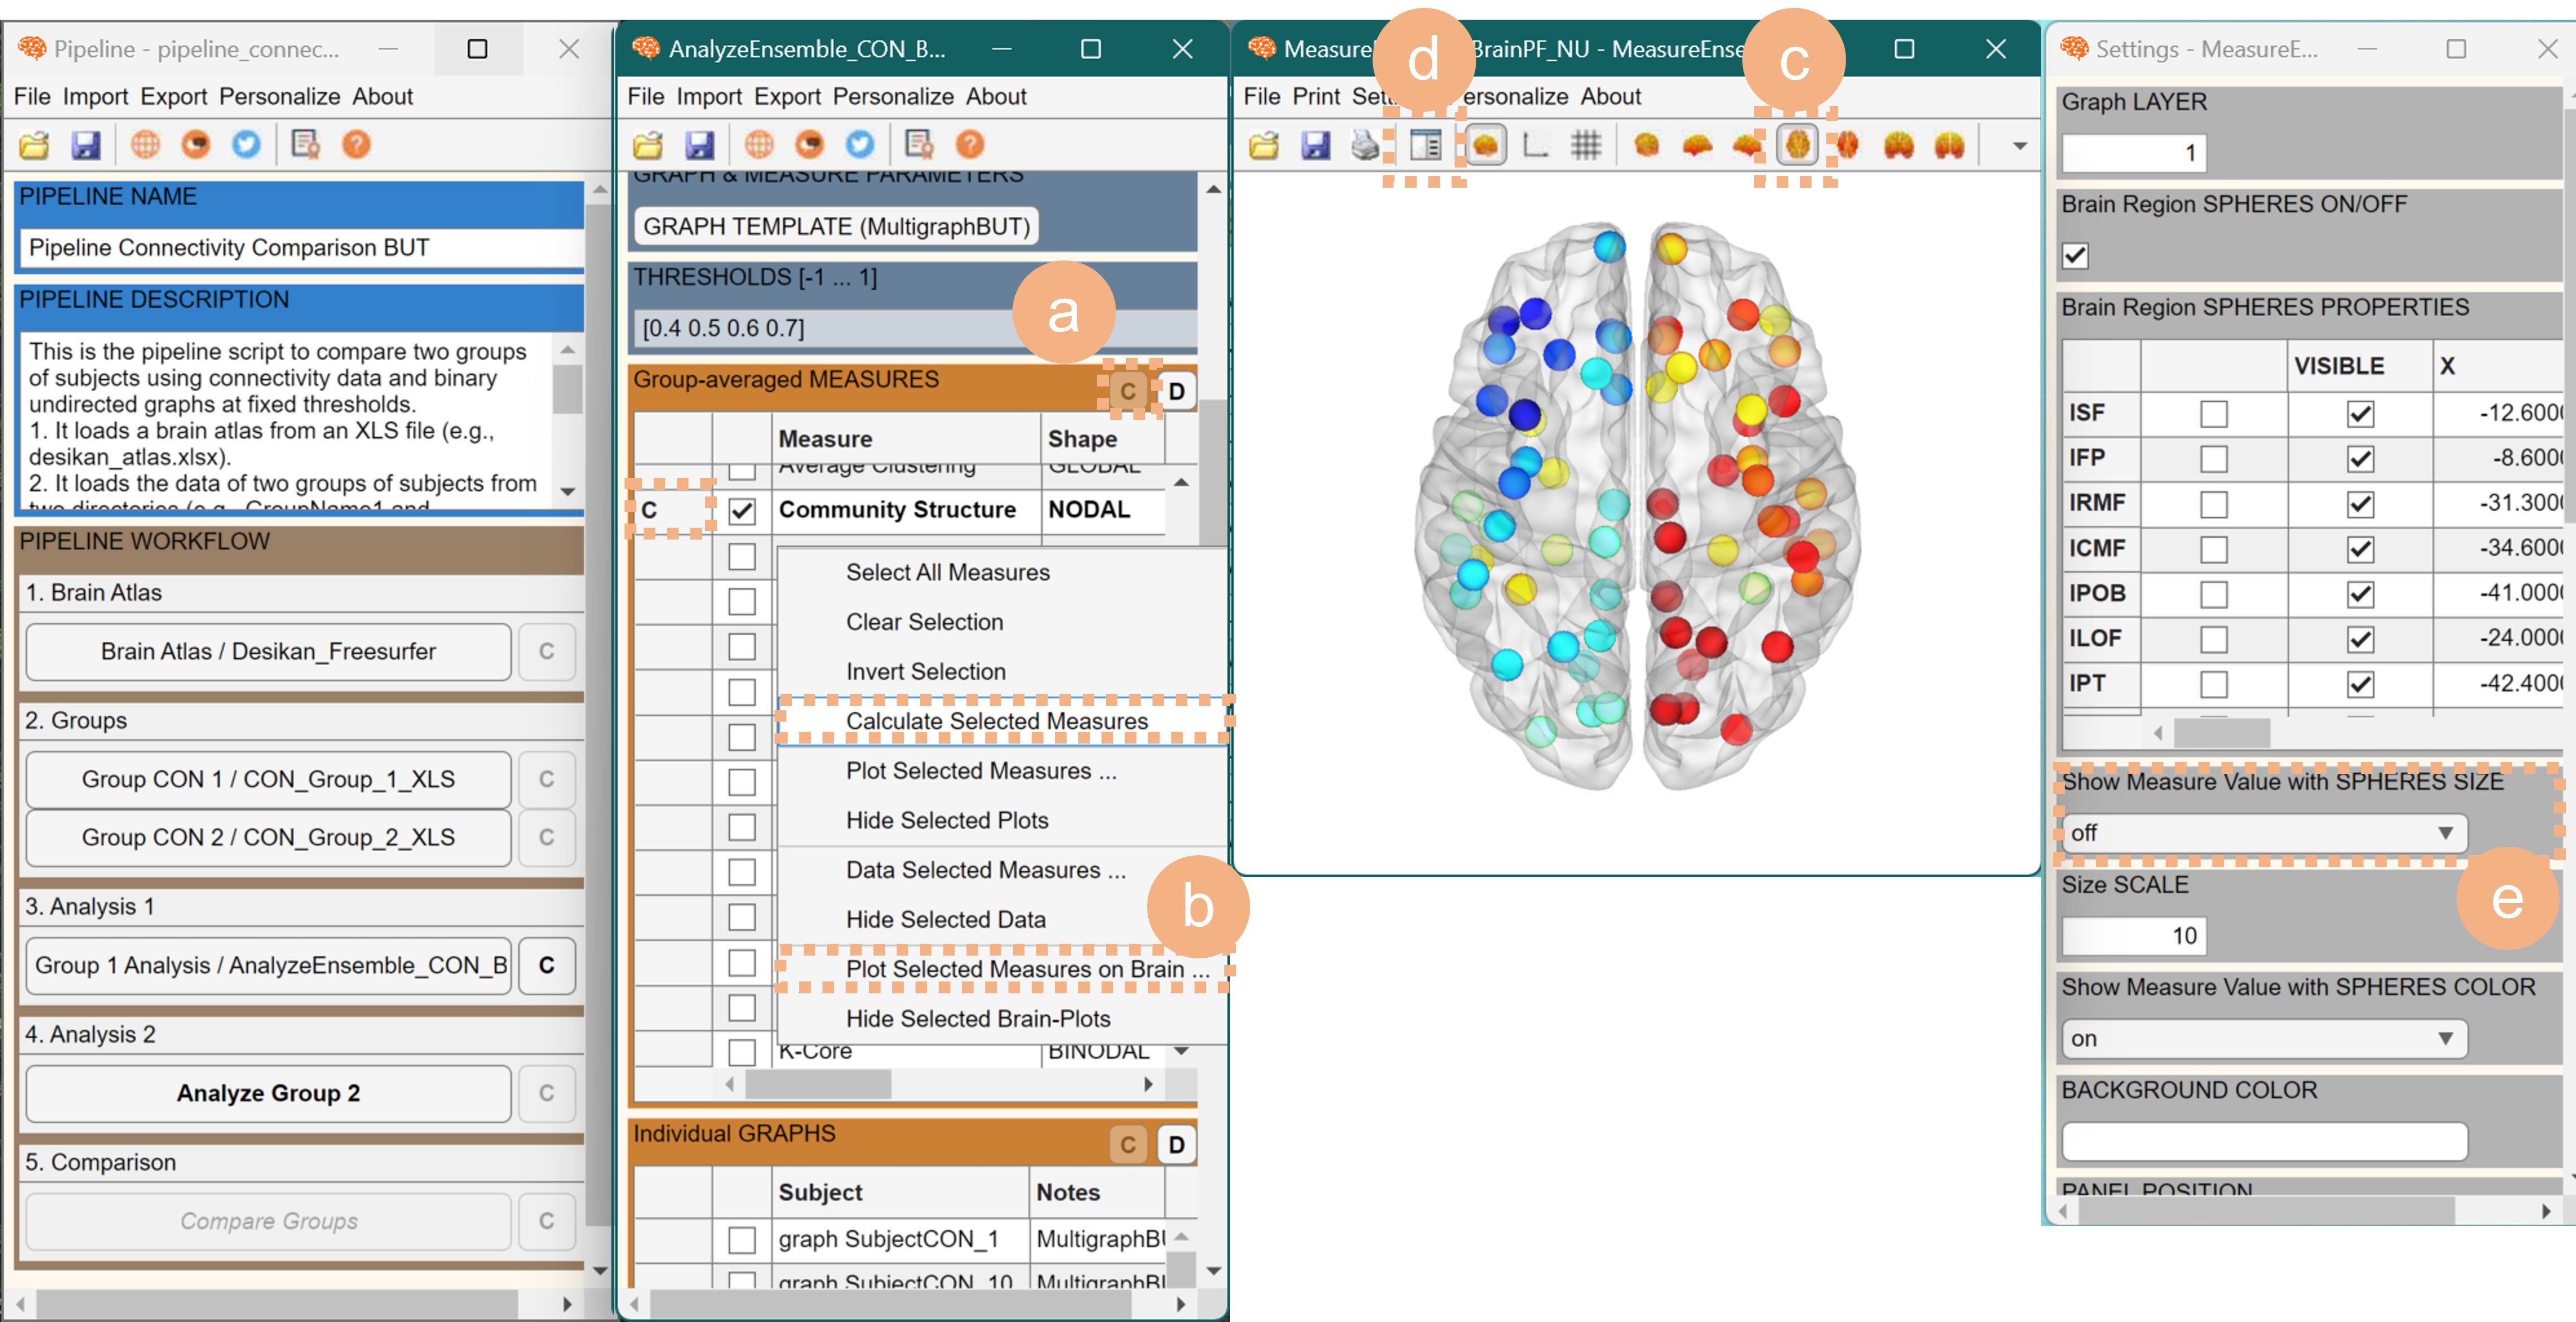
\includegraphics{fig05.jpg}
	}
	{Analyze the Group Data}
	{
	{\bf a} Click on \fn{Analyze Group 1} in the pipeline's GUI.
	{\bf b} In this new window, you can select the statistical test fo the correlations {\bf c}, what you want to do with the negative correlation weights {\bf d} and calculate some graph measures {\bf e}.
	}
 
\section{Step 4: Analysing the Data of Group 2}

After the analysis of group 1, you can proceed with the analysis of the second group by clicking on \fn{Analyze Group 2}. You will notice that, in the new window that is shown, the parameters you selected for group 1 are already selected and fixed for this analysis. If you realize that some of the options you previously selected are not the ones you would like, you can reset the analysis parameters of group 1 by clicking on the C checkbox next to it.

\section{Step 5: Comparing Groups}

Once you have explored the network measures for each group, you can proceed with their statistical comparison. To do this, you should click on \fn{Compare Groups} (\Figref{fig:06}a) and in the new window select if you want a waiting bar and verbose functions ON while you wait for the analysis to finish {\Figref{fig:06}b}. You can also decide how many permutations you want to use to assess differences between groups {\Figref{fig:06}c} and, if the groups are not independent but represent the same subjects in two different points in time, you can select the longitudinal comparison option, which will permute the values within each subject {\Figref{fig:06}d}. Finally, you can select the graph measures you want to compare between groups {\Figref{fig:06}e} and once you have selected all the measures you are interested in, you should right click and select \fn{Calculate all selected comparisons} {\Figref{fig:06}f}. If you turn ON the wait bar and verbose functions, two window bars will open that show you at which point in time the analysis is. There is one last option on this GUI that you can select to save intermediate results during the permutations.

	\fig{figure}
	{fig:06}
	{
	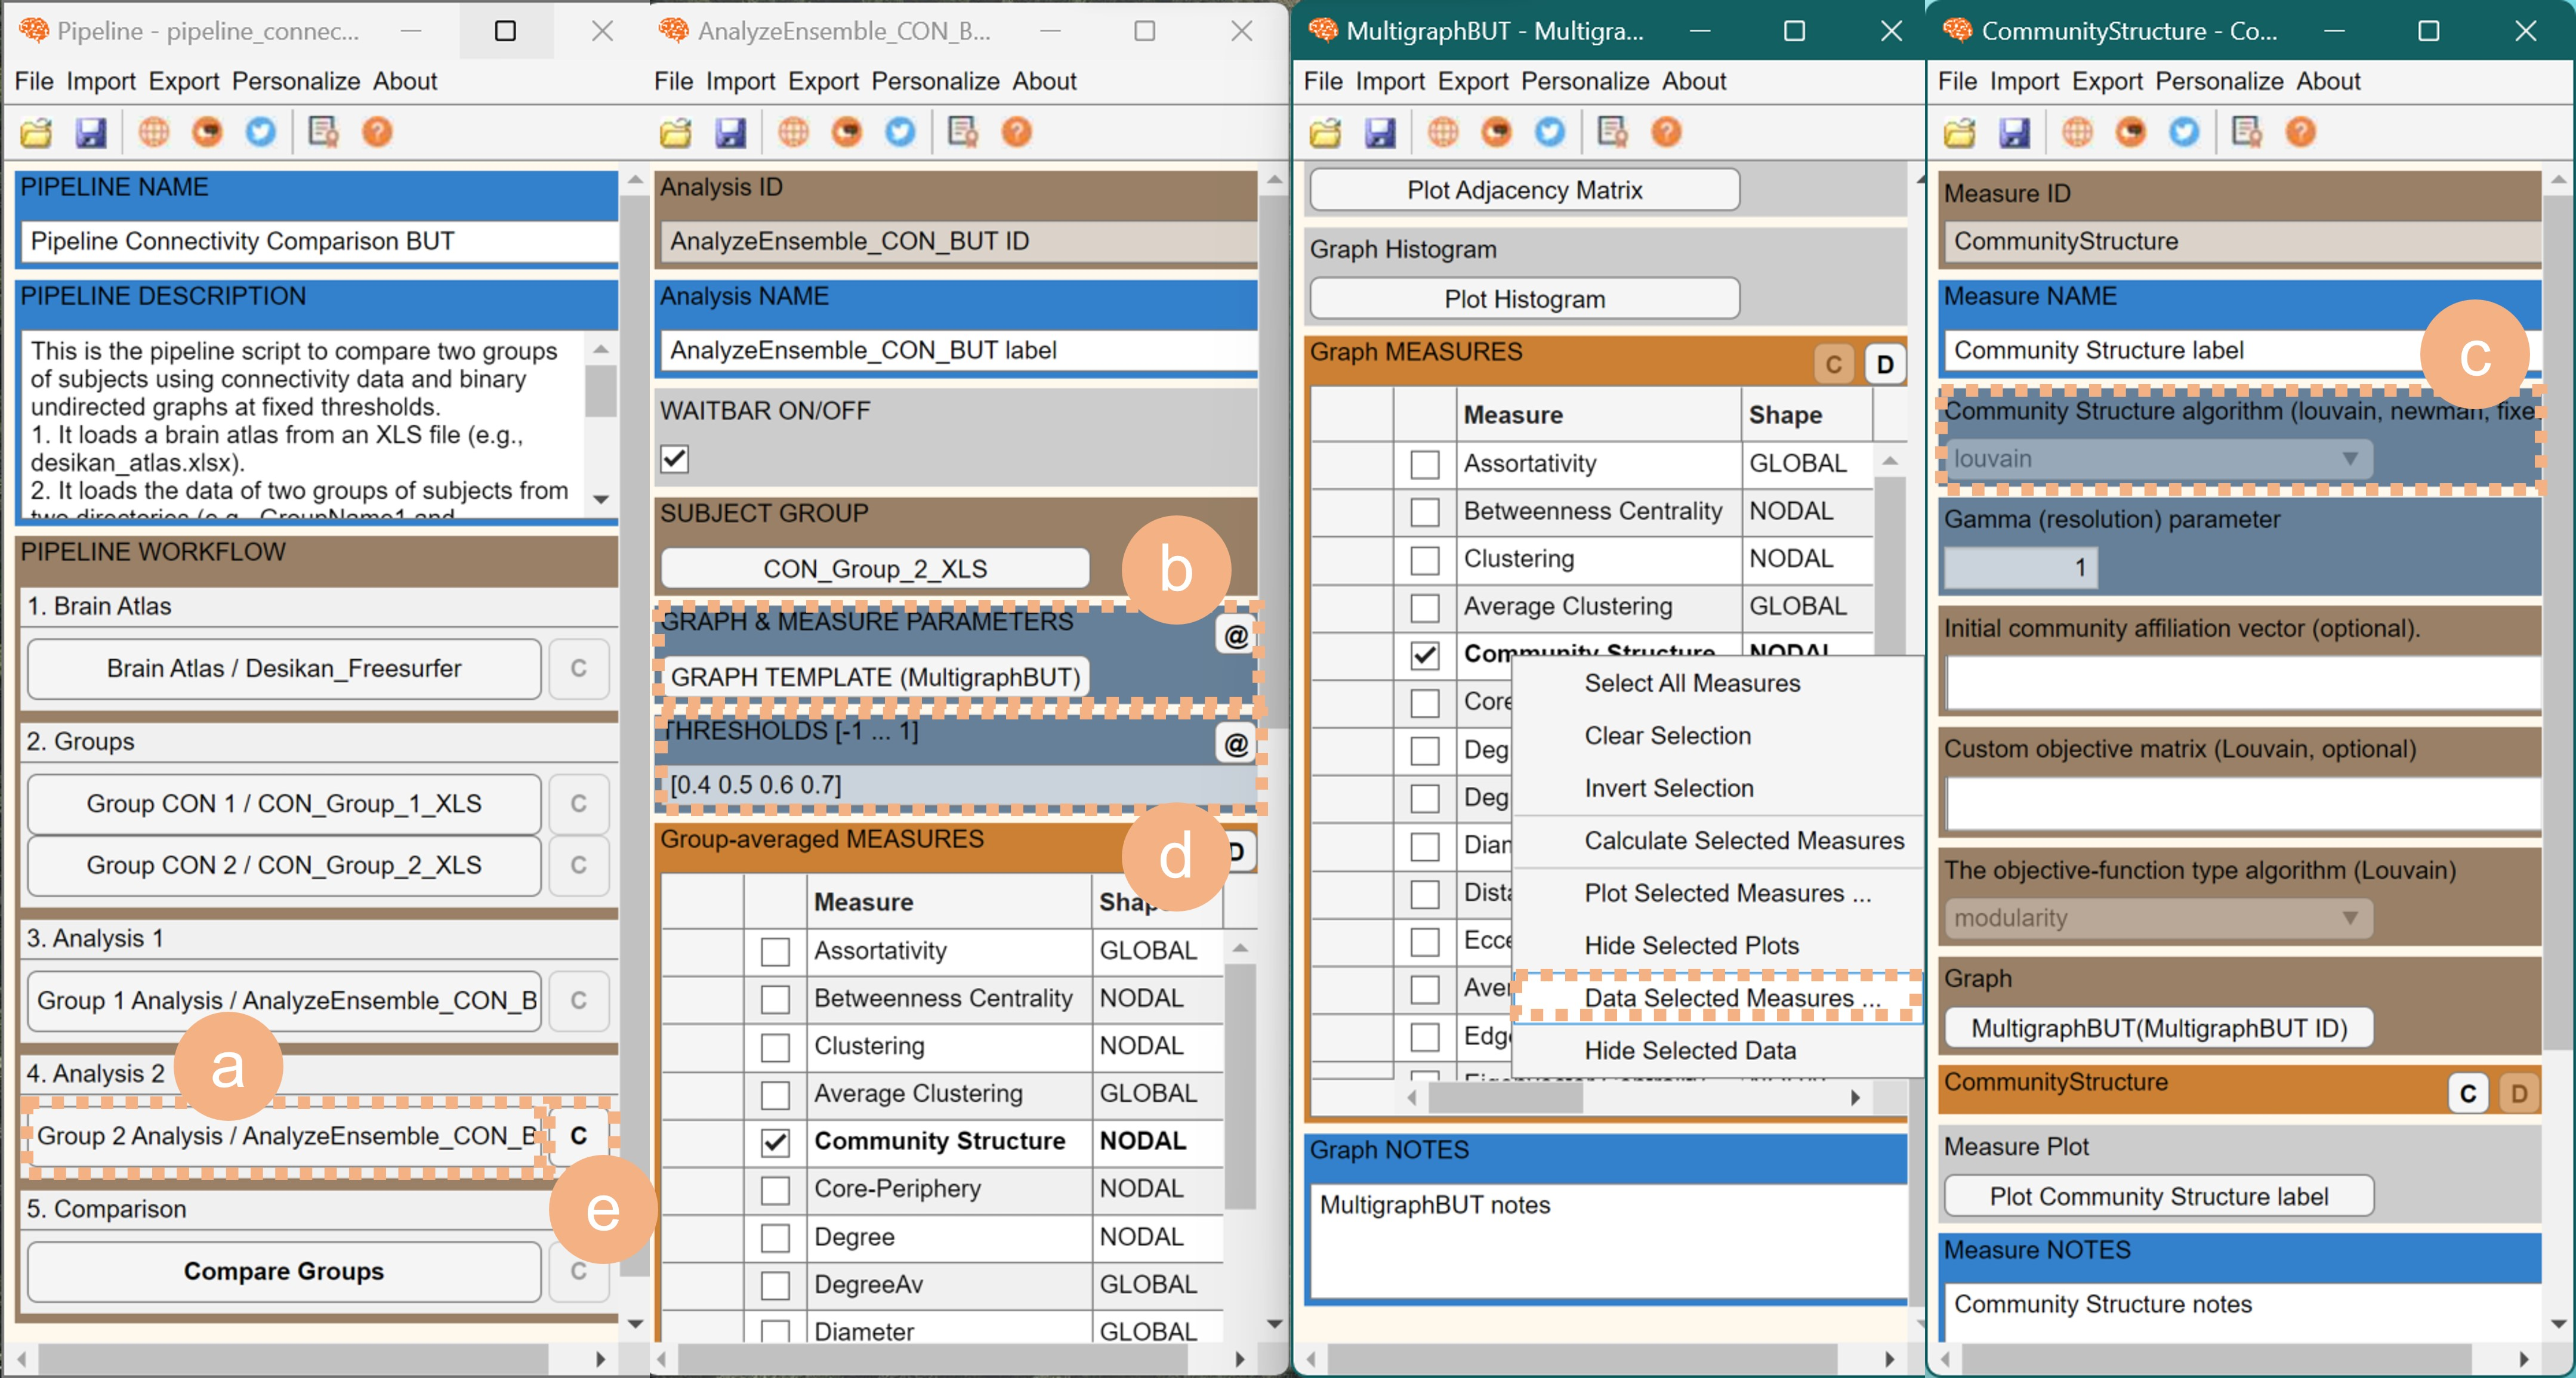
\includegraphics{fig06.jpg}
	}
	{Compare the Group Data}
	{
	{\bf a} Click on \fn{Compare Groups} in the pipeline's GUI.
	{\bf b} In this new window, you can select what to turn ON/OFF the wait bar and verbose functions {\bf c}, you can change the number of permutations {\bf d}, whether to perform a longitudinal group comparison {\bf f}, compare some graph measures between groups {\bf e}, or memorize intermediate steps {\bf f}.
	}
\end{document}